\chapter{Implementación de la herramienta de Minería de Procesos}
\addcontentsline{toc}{chapter}{Implementación de la herramienta de Minería de Procesos}

Comparando las Figuras \ref{fig:DBA1516P2GA1} y \ref{fig:problemsDBA1516P2GA} vemos que el diagrama de la implementación propia y el original obtenido con Disco coinciden.

\begin{figure}[H]
    \centering
    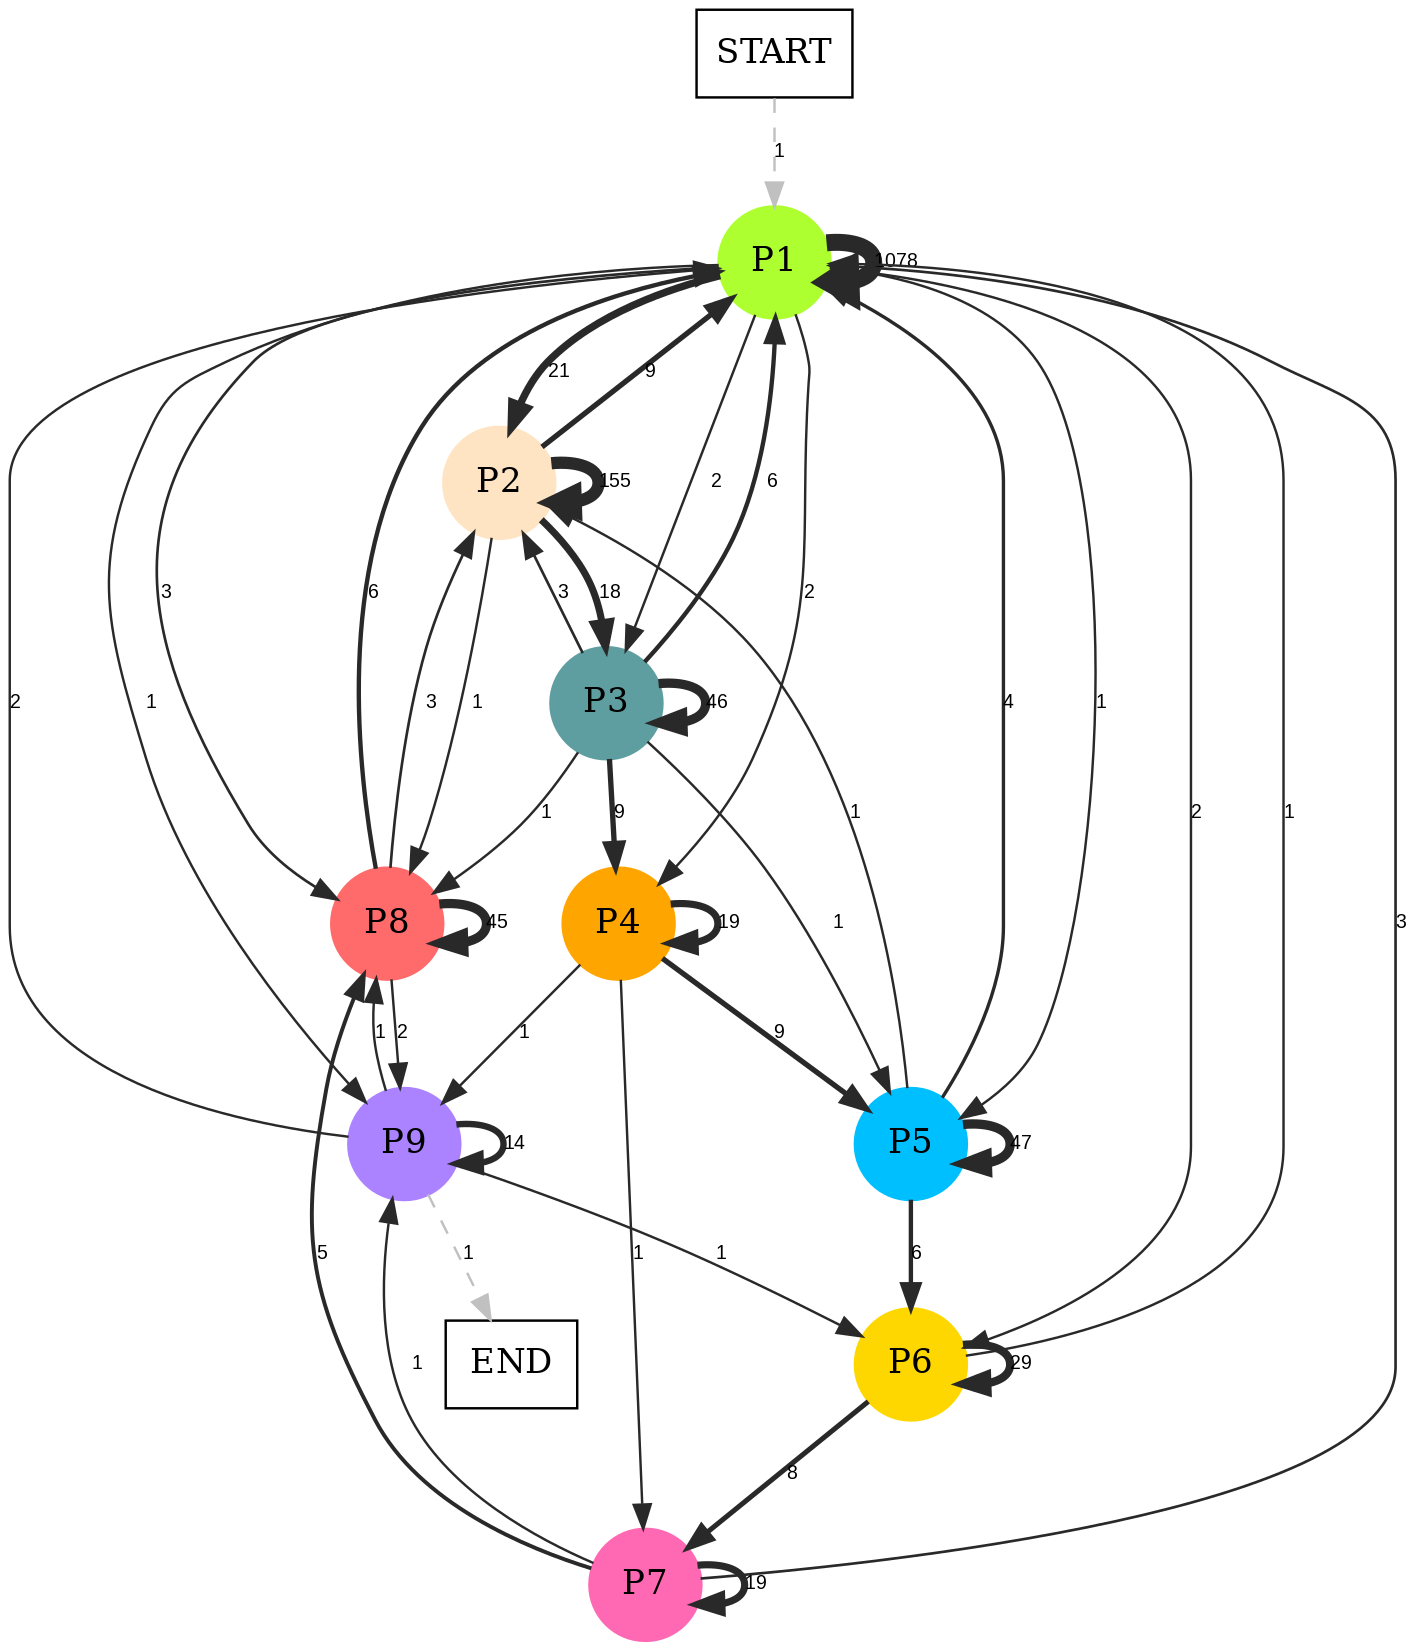
\includegraphics[width=0.5\textwidth]{DBA1516P2GA1.png}
    \caption{Análisis de procesos del grupo \texttt{DBA 1516 P2 GA} (\texttt{Activity} problema y \texttt{CaseId} grupo) obtenido con la implementación propia.}
    \label{fig:DBA1516P2GA1}
\end{figure}

Además, como podemos ver en la Figura \ref{fig:DBA1516P2GA2}, hemos obtenido el mismo diagrama que en el de la Figura \ref{fig:compoundDBA1516P2GA} con la salvedad de que hemos impedido el retorno a un estado anterior (el motivo se verá más adelante). Es decir, se han eliminado ciclos.

\begin{figure}[H]
    \centering
    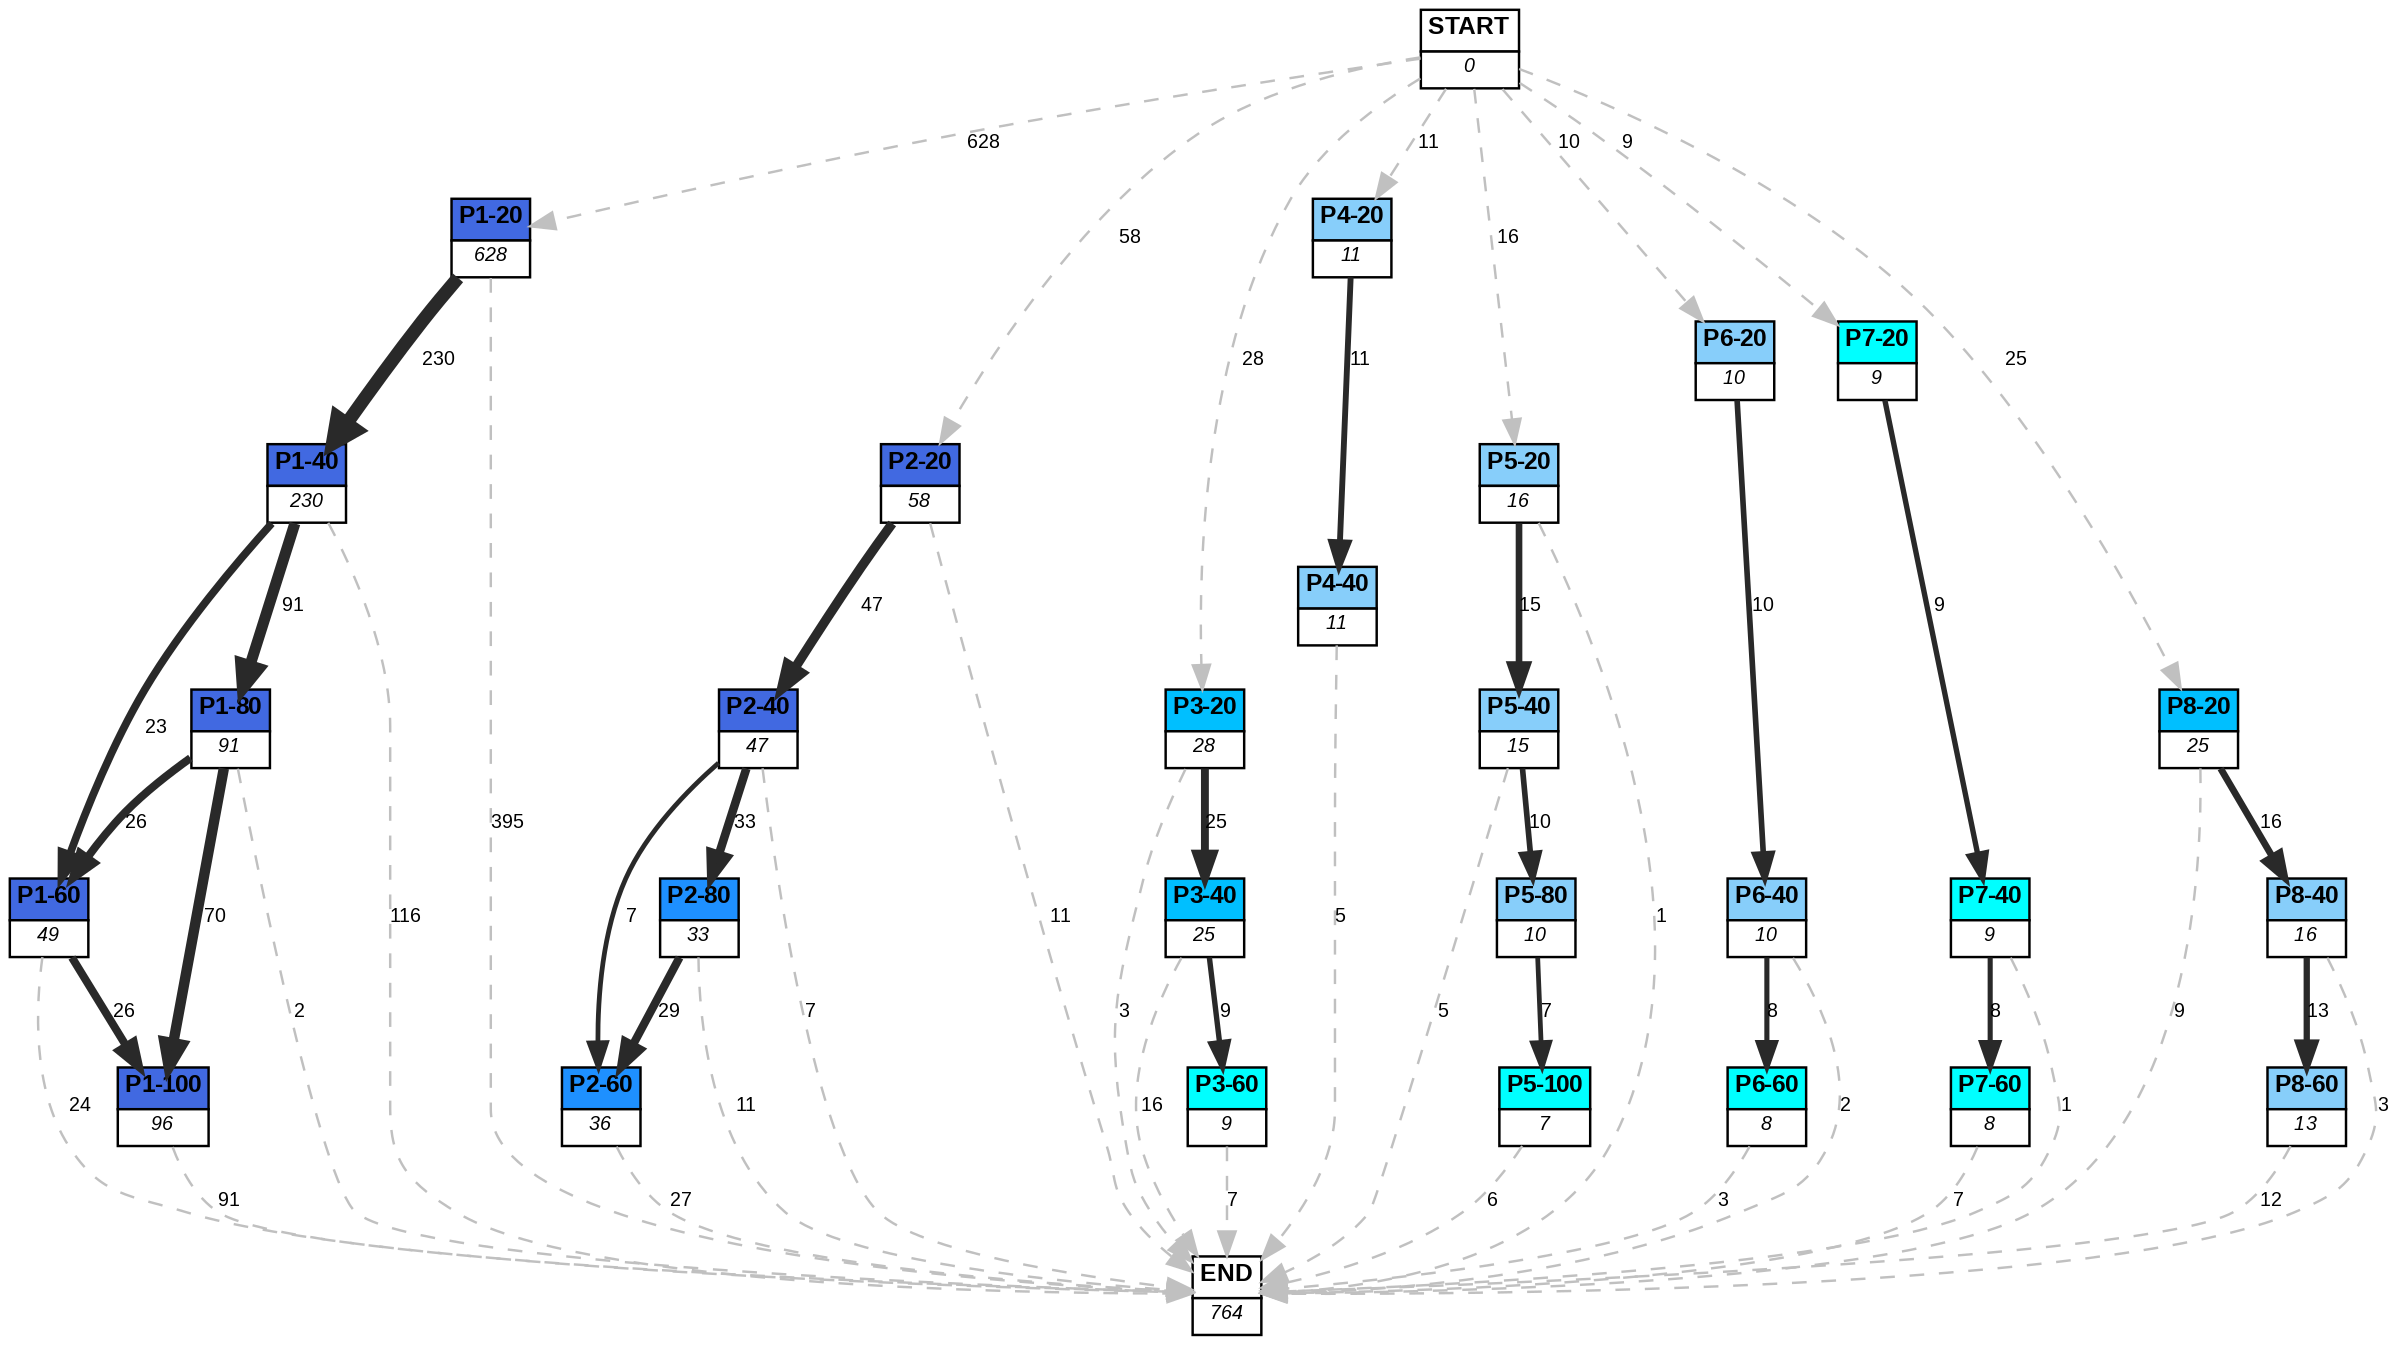
\includegraphics[width=\textwidth]{DBA1516P2GA2.png}
    \caption{Análisis de procesos del grupo \texttt{DBA 1516 P2 GA} (\texttt{Activity} problema-milestone y \texttt{CaseId} sesión) obtenido con la implementación propia.}
    \label{fig:DBA1516P2GA2}
\end{figure}

A partir de ahora, estos diagramos tendrán la consideración de grafos. En particular, serán grafos dirigidos y operaremos con ellos como tales. En el siguiente capítulo se expondrán los conceptos básicos de grafos y principales resultados matemáticos que se usarán en este trabajo fin de grado.